%!TEX root = ../Thesis.tex
\section{Grundlagen und Hintergrund}
Für die Umsetzung des Projekts ist theoretisches Wissen rund um Datenspeicherung -verarbeitung und -verteilung 
sowie Webdesign notwendig. Während grundlegendes Informatisches Fachwissen vorausgesetzt wird,
werden alle weiteren für das Verständnis dieser Arbeit relevanten Konzepte im Folgenden erläutert.
\subsection{Fixed-Schema Datenbanken}
Die Newport-Datenbank hat aufgrund ihrer großen Datenmenge und Nutzerbasis ein unveränderbares Schema.
Das bedeutet, dass die vorgegebenen Spalten nicht bearbeitet, und auch keine neuen Spalten hinzugefügt werden können.
Dadurch wird verhindert, dass die Anzahl an Spalten der Datenbank unkontrolliert wächst, was sich negativ auf Recheneffizienz
und Übersichtlichkeit auswirken könnte. \footnote{quelle bitte}
Ein Nachteil dieses Konzepts ist jedoch die geringere Flexibilität. Ohne die Möglichkeit, neue Spalten hinzuzufügen, 
sind Nutzer auf die zum Zeitpunkt der Erstellung der Datenbank vorgesehenen Informationen beschränkt.
Im Rahmen dieses Projekt soll diese Flexibilität durch Verwendung des \"Attribute-Value-Pair\"-Modells in einer umschließenden
Architektur gewährleistet werden, ohne aber die Vorteile einer Fixed-Schema Datenbank zu mindern
\subsection{Attribute-Value-Pair Modell}
Im Rahmen des Attribute-Value-Pair Modells (In Zukunft AVPM) werden Attribute, durch welche ein Objekt genauer beschrieben wird,
in eine eigenständige Tabelle ausgegliedert. Diese Tabelle ist über einen Fremdschlüssel mit dem jeweils tragenden Objekt verbunden.
Die Attribute sind in der Tabelle als Schlüssel-Wert-Paare gespeichert. Diese Struktur ermöglicht eine flexible Erweiterung der Attribute,  
ohne dass die Struktur der Datenbank verändert werden muss: \break
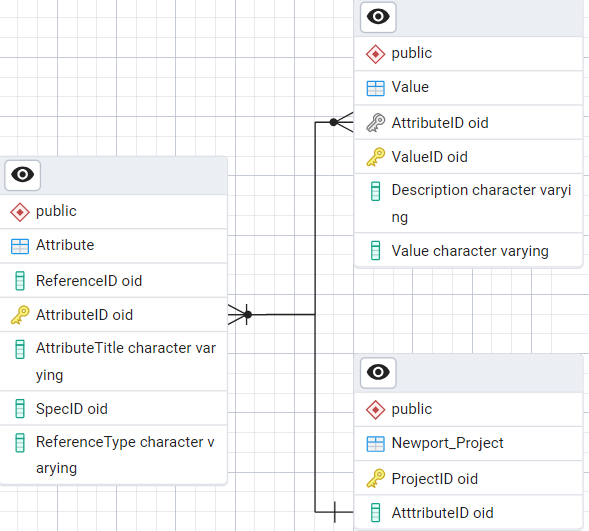
\includegraphics{./img/avpmGraphic.png}
\subsection{Technologischer Rahmen}
Um dieses Modell im Backend umzusetzen, und dann im Front-End nutzbar zu machen, bedarf es verschiedener Technologien.
Im Backend werden die Daten in einer Aurora PostgreSQL Datenbank gespeichert\footnote{Diese Wahl beruht auf Standards im Unternehmen. Dazu mehr in der Evaluierung}. 
Aurora PostgreSQL (Im Folgenden Aurora) ist ein Dienst, der die Erstellung von relationalen Datenbanken ermöglicht. Auf dieser relationalen Datenbank ermöglicht eine 
in NodeJS \footnote{Bessere Kompatibilität mit React als alternativen} erstellte API den Zugriff auf und die Bearbeitung der gespeicherten Daten.
Auf diese API greift dann widerum eine React-App zu, die dann ermöglicht, durch eine Benutzeroberfläche die API zur Kommunikation mit der Datenbank zu benutzen.
Die Architektur ist bewusst mehrgliedrich gehalten, um Erweiterungen wie Daten-Redundanz zu ermöglichen \footnote{Unter anderem sollen die Daten in ein großes Daten
Warehouse der Bayer Cropscience kopiert werden} Die Wahl dieses technologischen Rahmens beruht auf vorhandenem Wissen und Infrastruktur im Unternehmen, sowie auch 
Abwägung der Entwicklungsgeschwindigkeit. Grundsätzlich stehen Enwticklern in der Web-Entwicklung jedoch viele Möglichkeiten zur Verfügung
\subsection{Alternative Technologien}
Für die Datenbank wäre es denkbar gewesen, anstatt einer relationalen auf eine sogenannte NoSQL Datenbanken zurückzugreifen. Eine solche Lösung
wird auch im AWS-System angeboten. Der Grund, warum sich gegen diese Option entschieden wurde, liegt in der Natur der Datengrundlage. NoSQL eignet sich vor allem für 
große Mengen unstrukturierter Daten, während traditionelle Datenbanken besser mit strukturierten Daten umgehen können \footnote{nosql source}
Im Rahmen der Anwendung muss zwingendermaßen eine strenge Typisierung von Daten gegeben sein, da auf dessen Basis unter anderem Grafiken erstellt werden sollen. 
Aus diesem Grund ist eine strukturierte Datenbank für den speziellen Zweck des Projekts besser geeignet. 
\break
Die Entscheidung, NodeJS für die API zu verwenden, beruht hauptsächlich auf der zeitlichen Komponente der Entwicklung. React basiert auf einem NodeJS-Environment, weshalb
es sich anbietet, die gleiche Umgebung für die APi zu verwenden. Grundsätzlich hätte auch jede andere Umgebung zur API-Erstellung ihren Zweck erfüllt, und diese Entscheidung 
beruht eher auf Bequemlichkeit. React hingegen als Umgebung wurde mit dem Hintergedanken der Modularität gewählt. Da das Projekt nicht nur eine einzene Anwendung, sondern eher 
einen Komplex kleinerer Tools beherbergen soll, bietet sich ein modulares Framework wie React an, wodurch dieses schon zu Beginn als Anforderung feststand, und als Basis 
aller weiteren Entscheidungen verwendet wurde. Zudem wird React unternehmensintern immer häufiger für verschiedenste Anwendungen verwendet, weshalb die Infrastruktur für das 
Deployment bereits aufgebaut ist. 
